\documentclass[tikz,border=10pt]{standalone}
\usepackage{pgf}
\usepackage{xcolor}
\usetikzlibrary{arrows,automata,positioning}

\definecolor{statecolor}{HTML}{e89a6f} 
\definecolor{actioncolor}{HTML}{bcd35f} 

\tikzset{
    state/.style={
        shape=rectangle,
        draw=black,
        fill=statecolor,
        align=center,
        minimum height=2em,
        minimum width=4em,
        inner sep=2pt
    },
    action/.style={
        shape=rectangle,
        draw=black,
        fill=actioncolor,
        align=center,
        inner sep=10pt,
        rounded corners=15pt,
    },
    reward/.style={
    	|->,
    	decoration={snake, amplitude=1.5mm, segment length=3mm},
    	decorate,
    	postaction={draw, line width=1pt, shorten <=1pt, -{Stealth[scale=1.5]}}
    },
    transition/.style={
    	->,
    }
}

\begin{document}
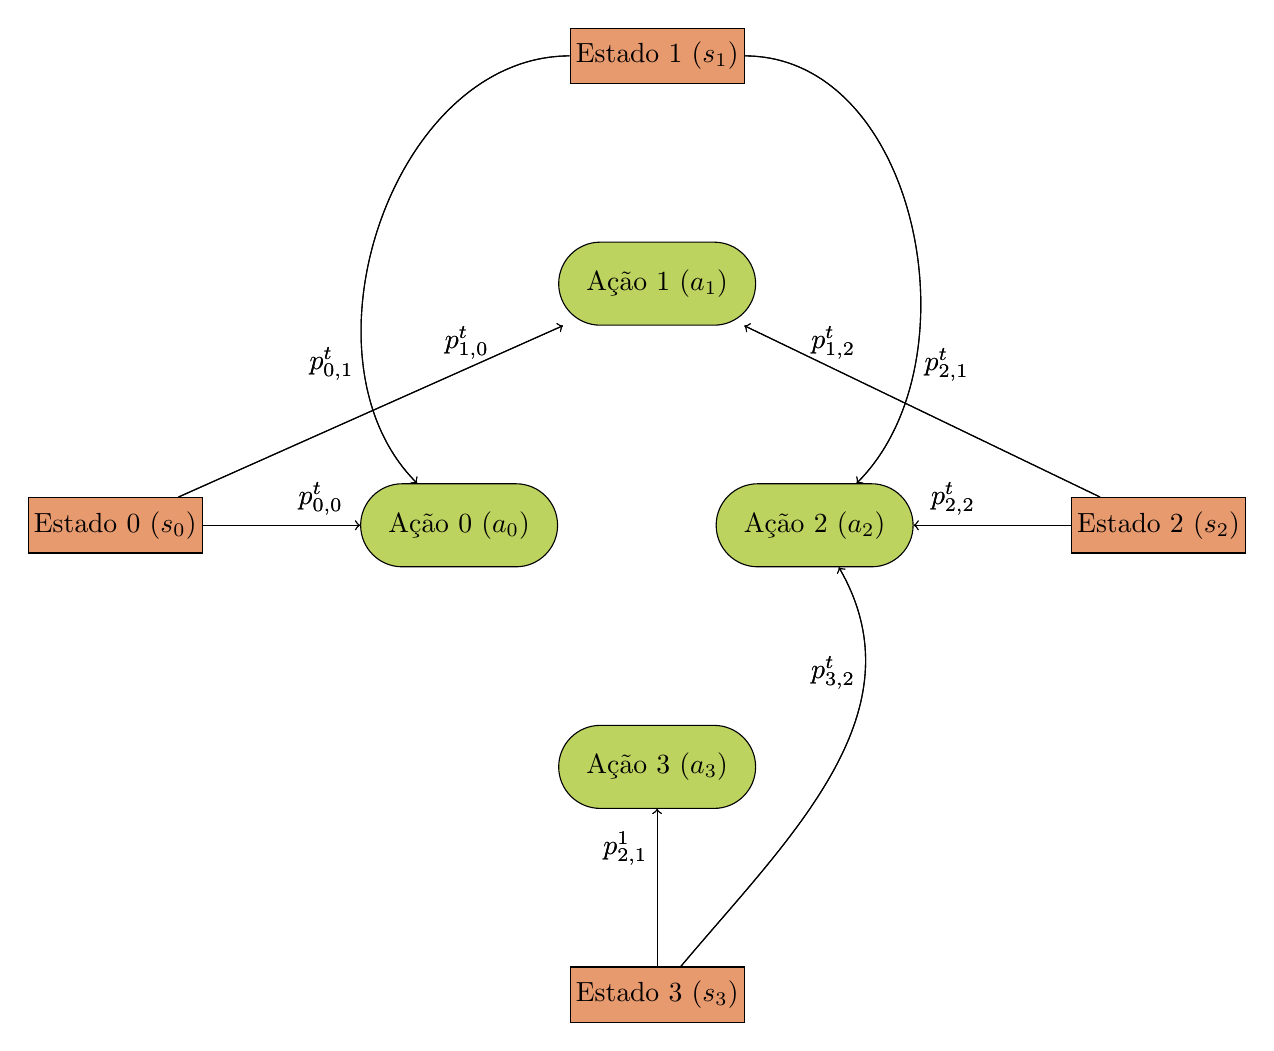
\begin{tikzpicture}
    \node[state] (s0) {Estado 0 ($s_0$)};
    
    \node[action, right=2cm of s0] (a0) {Ação 0 ($a_0$)};
    \node[action, above right=2cm and 0cm of a0] (a1) {Ação 1 ($a_1$)};
    \node[action, right=2cm of a0] (a2) {Ação 2 ($a_2$)};
    \node[action, below right=2cm and 0cm of a0] (a3) {Ação 3 ($a_3$)};
    
    \node[state, above=2cm of a1] (s1) {Estado 1 ($s_1$)};
    \node[state, right=2cm of a2] (s2) {Estado 2 ($s_2$)};
    \node[state, below=2cm of a3] (s3) {Estado 3 ($s_3$)};
    
    \begin{scope} % actions
    	\draw[transition] 
    	(s0) 
    	to node[near end, above] {$p_{0,0}^{t}$} 
    	(a0);
    	
    	\draw[transition] 
    	(s0) 
    	to node[near end, above] {$p_{1,0}^{t}$} 
    	(a1);
    	
    	\draw[transition] 
    	(s1) 
    	to[in=45, out=360] node[near end, right] {$p_{2,1}^{t}$} 
    	(a2);
    	
    	\draw[transition] 
    	(s1) 
    	to[in=135, out=180] node[near end, left] {$p_{0,1}^{t}$} 
    	(a0);
    	
    	\draw[transition] 
    	(s2) 
    	to node[near end, above] {$p_{1,2}^{t}$} 
    	(a1);
    	
    	\draw[transition] 
    	(s2) 
    	to node[near end, above] {$p_{2,2}^{t}$} 
    	(a2);
    	
    	\draw[transition] 
    	(s3) 
    	to node[near end, left] {$p_{2,1}^{1}$} 
    	(a3);
    	
    	\draw[transition] 
    	(s3) 
    	to[in=300, out=50] node[near end, left] {$p_{3,2}^{t}$} 
    	(a2);
    \end{scope}
    \begin{scope} % rewards
    	\draw[transition] 
    	(s0) 
    	to node[near end, above] {$p_{0,0}^{t}$} 
    	(a0);
    	
    	\draw[transition] 
    	(s0) 
    	to node[near end, above] {$p_{1,0}^{t}$} 
    	(a1);
    	
    	\draw[transition] 
    	(s1) 
    	to[in=45, out=360] node[near end, right] {$p_{2,1}^{t}$} 
    	(a2);
    	
    	\draw[transition] 
    	(s1) 
    	to[in=135, out=180] node[near end, left] {$p_{0,1}^{t}$} 
    	(a0);
    	
    	\draw[transition] 
    	(s2) 
    	to node[near end, above] {$p_{1,2}^{t}$} 
    	(a1);
    	
    	\draw[transition] 
    	(s2) 
    	to node[near end, above] {$p_{2,2}^{t}$} 
    	(a2);
    	
    	\draw[transition] 
    	(s3) 
    	to node[near end, left] {$p_{2,1}^{1}$} 
    	(a3);
    	
    	\draw[transition] 
    	(s3) 
    	to[in=300, out=50] node[near end, left] {$p_{3,2}^{t}$} 
    	(a2);
    \end{scope}
\end{tikzpicture}
\end{document}

